
\subsection{Iteración 3}

En la última iteración de esta entrega se ha buscado poner a prueba la adaptación de varias personas al uso de la realidad virtual en general y en concreto a las mecánicas desarrolladas en esta entrega. Se ha hecho hincapié en la facilidad de uso y la comodidad del usuario durante el juego. 

Para esto se ha desarrollado una pequeña escena de prueba en la que primero el jugador debe adoptar una postura corporal de forma que se activen de forma correcta unos triggers preparados previamente y que cambian cada 10 segundos hasta 3 veces. A continuación, el usuario se encuentra ante una mesa virtual (figura \ref{fig:E2_mesa}) en la que encuentra varios objetos, dos cubos verdes y dos cubos azules. En los bordes de la mesa hay 4 plataformas de los mismos colores que los cubos. El jugador puede interactuar libremente con estos objetos, pero debe colocar cada cubo en una plataforma de su color correspondiente. Una vez realizada la tarea, debe pulsar el botón situada en la parte derecha de la mesa. La pulsación de este botón provoca que se reproduzca un sonido proveniente de la parte trasera del usuario. Finalmente, el jugador tiene que girarse para ver la fuente del sonido y terminar así la prueba.


\begin{figure}
  \centering
    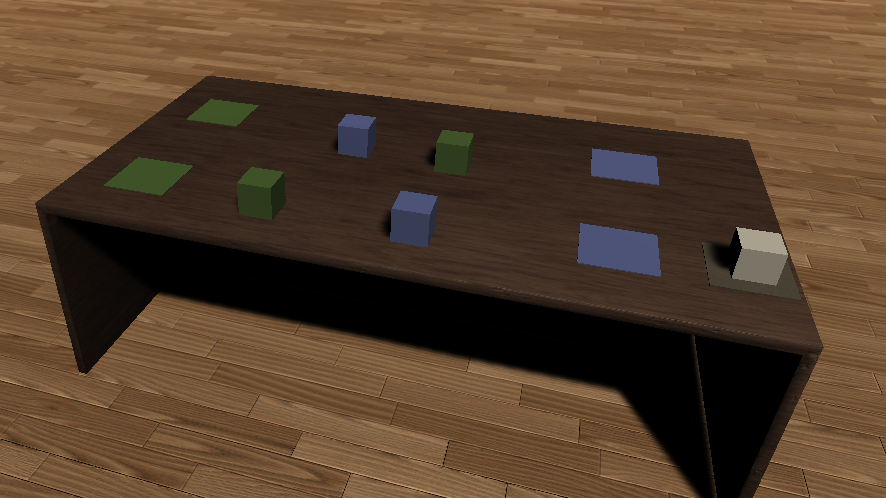
\includegraphics[width=0.5\textwidth]{04.Desarrollo/02.Entrega2/03.Iteracion2_3/00.Figuras/01.mesa.png}
    \caption{Mesa con objetos de prueba para las interacciones básicas, snap zones y botones.}
    \label{fig:E2_mesa}
\end{figure}




Esta prueba se ha realizado con varias personas mientras se monitorizaba mediante Unity todos los resultados y el funcionamiento de las mecánicas. Han participado tres personas que se caracterizan de la siguiente forma:

\begin{itemize}
    \item{Persona mayor de 50 años con poca experiencia tecnológica y ninguna experiencia en RV.}
    \item{Persona entre 20 y 25 años, con experiencia tecnológica, pero sin experiencia en RV.}
    \item{Persona entre 20 y 25 años con gran experiencia tanto en tecnología como en RV.}
\end{itemize}




Tras guiar a estas tres personas durante la prueba y posteriormente entrevistarlas sobre su experiencia se han obtenido información útil para el desarrollo del proyecto y que se expone a continuación.

\begin{itemize}

\item{Todas las personas han necesitado un breve periodo de adaptación a la realidad virtual, en el caso de las personas jóvenes ha sido más corto y ha consistido principalmente en ajustes físicos del casco de realidad virtual como la tensión se sus amarres o la distancia focal de las lentes para evitar ver de forma borrosa. En la persona mayor ha sido necesario más tiempo para adaptarse al entorno virtual, pero no provocando mareo ni otros efectos perjudiciales.}
\item{Aunque ninguna persona ha tenido dificultades en seguir la prueba de posiciones, se ha observado que es necesario reajustar el tamaño y posición de los triggers, así como su cantidad y separación.}
\item{En el uso de las manos virtuales las dos personas sin experiencia en RV prefieren que el avatar muestre una representación virtual del mando que están sosteniendo para facilitar la inmersión. Sin embargo, a la hora de interactuar y coger objetos han encontrado más difícil utilizar el avatar con mando por la discordancia con el mundo real en el que no se puede coger otro objeto mientras ya se tiene uno sujeto. La persona con experiencia en RV ha preferido el avatar sin representación del mando en todo momento. Por tanto, se concluye que el mando virtual es útil para crear una inmersión inicial, pero debe ser sustituido cuando llega el momento de realizar interacciones con las manos.}
\item{Durante la prueba de agrupación de los objetos por colores, las dos personas sin experiencia en RV han tenido ligeros inconvenientes a la hora de coger objetos principalmente por la estimación de la distancia a la que se encuentran. Estos inconvenientes no han sido graves y ambas personas se han acostumbrado rápidamente.}
\item{Llegado el momento de intentar localizar la posición de la fuente de sonido a sus espaldas todo el mundo ha tenido problemas en discernir de dónde procedía el sonido. Tras investigar el problema es posible que por la naturaleza del audio digital y el dispositivo de reproducción usado sea difícil distinguir entre ciertas posiciones de una fuente como por ejemplo detrás del jugador o justo sobre su cabeza. Por lo tanto, esta prueba deberá ser acotada para que la fuente de sonido solo pueda apareces en lugares en los que sea posible localizarla de forma cómoda.}

\end{itemize}


